% Báo cáo Bài tập lớn IoT và Ứng dụng - Nhóm 13
% Biên dịch: xelatex main.tex (chạy 2 lần để có mục lục) hoặc `make`
\documentclass[12pt,a4paper]{extarticle}
% Cỡ chữ thân bài 13pt
\makeatletter\renewcommand{\normalsize}{\@setfontsize\normalsize{13}{15.6}}\makeatother

% ---------------------------------------------------------------------------
% Gói và phông chữ
% ---------------------------------------------------------------------------
\usepackage{fontspec}
\setmainfont{Times New Roman}
\setmonofont{Menlo}[Scale=0.82]
\usepackage[left=3cm,right=2cm,top=2.5cm,bottom=2.5cm]{geometry}
\usepackage{setspace}
\setstretch{1.3}
\setlength{\parindent}{1cm}
\setlength{\parskip}{3pt}
\usepackage{indentfirst}

\usepackage{graphicx}
\usepackage{float}
\usepackage{array}
\usepackage{tabularx}
\usepackage{longtable}
\usepackage{booktabs}
\usepackage{multirow}
\usepackage[table]{xcolor}
\usepackage{enumitem}
\usepackage{titlesec}
\usepackage{caption}
\usepackage{listings}
\usepackage{fancyhdr}
\usepackage{tikz}
\usetikzlibrary{arrows.meta,positioning,shapes.geometric,shapes.misc,fit,calc,backgrounds}
\usepackage[hidelinks,unicode]{hyperref}

\graphicspath{{hinh/}}

% ---------------------------------------------------------------------------
% Thông tin nhóm (sửa tại đây)
% ---------------------------------------------------------------------------
\newcommand{\TenDeTai}{HỆ THỐNG NHÀ THÔNG MINH IoT DÙNG ESP32,\\ TRỢ LÝ GIỌNG NÓI VÀ NHẬN DIỆN KHUÔN MẶT}
\newcommand{\TenDeTaiThuong}{Hệ thống nhà thông minh IoT dùng ESP32, trợ lý giọng nói và nhận diện khuôn mặt}
\newcommand{\HocPhan}{IoT và Ứng dụng}
\newcommand{\GiangVien}{TS. Lê Văn Vịnh}
\newcommand{\NhomBTL}{13}
\newcommand{\NamBaoCao}{2026}

% ---------------------------------------------------------------------------
% Tiêu đề mục: I. / 1.1. / 1.1.1.
% ---------------------------------------------------------------------------
\renewcommand{\thesection}{\Roman{section}}
\renewcommand{\thesubsection}{\arabic{section}.\arabic{subsection}}
\renewcommand{\thesubsubsection}{\thesubsection.\arabic{subsubsection}}
\titleformat{\section}{\normalfont\fontsize{14}{17}\bfseries}{\thesection.}{0.5em}{\MakeUppercase}
\titleformat{\subsection}{\normalfont\fontsize{13}{16}\bfseries}{\thesubsection.}{0.5em}{}
\titleformat{\subsubsection}{\normalfont\fontsize{13}{16}\bfseries\itshape}{\thesubsubsection.}{0.5em}{}
\titlespacing*{\section}{0pt}{14pt}{8pt}
\titlespacing*{\subsection}{0pt}{10pt}{4pt}
\titlespacing*{\subsubsection}{0pt}{8pt}{3pt}

% Mục lục: "I. ...", "1.1. ..." có dòng chấm; danh mục "Hình 1: ..."
\usepackage{titletoc}
\newcommand{\chamtoc}{\titlerule*[0.55pc]{.}\contentspage}
\titlecontents{section}[0em]{\addvspace{3pt}}{\thecontentslabel.\ \ }{}{\chamtoc}
\titlecontents{subsection}[1.5em]{}{\thecontentslabel.\ \ }{}{\chamtoc}
\titlecontents{subsubsection}[3em]{}{\thecontentslabel.\ \ }{}{\chamtoc}
\titlecontents{figure}[0em]{}{Hình \thecontentslabel:\ }{}{\chamtoc}
\titlecontents{table}[0em]{}{Bảng \thecontentslabel:\ }{}{\chamtoc}
\setcounter{tocdepth}{3}

% Tên tiếng Việt
\renewcommand{\contentsname}{MỤC LỤC}
\renewcommand{\listfigurename}{DANH MỤC HÌNH ẢNH}
\renewcommand{\listtablename}{DANH MỤC BẢNG BIỂU}
\renewcommand{\refname}{TÀI LIỆU THAM KHẢO}
\renewcommand{\figurename}{Hình}
\renewcommand{\tablename}{Bảng}
\captionsetup{labelsep=colon,font=small,justification=centering}
\captionsetup[figure]{name=Hình}
\captionsetup[table]{name=Bảng,position=below}

% Mục không đánh số nhưng có trong mục lục
\newcommand{\mucchinh}[1]{%
  \section*{\centering #1}%
  \addcontentsline{toc}{section}{#1}}

% Danh sách
\setlist[itemize]{label=--,leftmargin=1.2cm,itemsep=1pt,topsep=3pt}
\setlist[enumerate]{leftmargin=1.2cm,itemsep=1pt,topsep=3pt}

% Bảng
\renewcommand{\arraystretch}{1.25}
\newcolumntype{L}{>{\raggedright\arraybackslash}X}
\newcolumntype{P}[1]{>{\raggedright\arraybackslash}p{#1}}
\newcolumntype{C}{>{\centering\arraybackslash}X}
\definecolor{tieude}{HTML}{DCE6F2}
\newcommand{\hang}{}  % hàng tiêu đề bảng: nền trắng

% Mã nguồn
\definecolor{nenma}{HTML}{F6F8FA}
\definecolor{chuthich}{HTML}{6A737D}
\definecolor{tukhoa}{HTML}{0033B3}
\definecolor{chuoi}{HTML}{067D17}
\lstset{
  basicstyle=\ttfamily\small\setstretch{1.0},
  backgroundcolor=\color{nenma},
  frame=single, rulecolor=\color{gray!40},
  keywordstyle=\color{tukhoa}\bfseries,
  commentstyle=\color{chuthich}\itshape,
  stringstyle=\color{chuoi},
  breaklines=true, columns=fullflexible, keepspaces=true,
  showstringspaces=false, tabsize=2,
  xleftmargin=3.4pt, xrightmargin=3.4pt, aboveskip=6pt, belowskip=4pt,
  extendedchars=true
}
\lstdefinelanguage{json}{
  morestring=[b]", stringstyle=\color{chuoi},
  literate={:}{{\textcolor{tukhoa}{:}}}1
}
\renewcommand{\lstlistingname}{Đoạn mã}

% Ảnh minh họa: có file trong hinh/ thì chèn, chưa có thì hiện khung chờ ảnh
\newcommand{\hinhanh}[3]{%
  \begin{figure}[H]\centering
  \IfFileExists{hinh/#1}{%
    \includegraphics[width=#3\linewidth,height=0.42\textheight,keepaspectratio]{#1}}{%
    \fbox{\parbox[c][5cm][c]{#3\linewidth}{\centering\itshape\color{gray}
      [Chèn ảnh: #2]\\[2pt]\small(đặt file \texttt{hinh/#1})}}}
  \caption{#2}
  \end{figure}}

% Kiểu TikZ dùng chung
\tikzset{
  khoi/.style={draw, rounded corners=3pt, align=center, fill=#1, minimum height=1cm, inner sep=5pt, font=\small},
  khoi/.default=white,
  muiten/.style={-{Stealth[length=2.2mm]}, thick},
  haichieu/.style={{Stealth[length=2.2mm]}-{Stealth[length=2.2mm]}, thick},
  nhan/.style={font=\scriptsize, align=center, fill=white, inner sep=1.5pt},
  quyetdinh/.style={draw, diamond, aspect=2.2, align=center, fill=yellow!15, font=\small, inner sep=1pt},
  buoc/.style={draw, rounded corners=2pt, align=center, fill=blue!6, font=\small, text width=#1, minimum height=0.8cm},
  buoc/.default=5.2cm,
}

% Đầu trang / chân trang
\pagestyle{fancy}
\fancyhf{}
\fancyfoot[C]{\thepage}
\renewcommand{\headrulewidth}{0pt}

\begin{document}

% ===========================================================================
% TRANG BÌA
% ===========================================================================
\begin{titlepage}
\newgeometry{left=2.5cm,right=2cm,top=2cm,bottom=2cm}
\begin{tikzpicture}[remember picture,overlay]
  \draw[line width=2.2pt] ($(current page.north west)+(2.2cm,-1.6cm)$) rectangle ($(current page.south east)+(-1.6cm,1.6cm)$);
  \draw[line width=0.6pt] ($(current page.north west)+(2.35cm,-1.75cm)$) rectangle ($(current page.south east)+(-1.75cm,1.75cm)$);
\end{tikzpicture}
\begin{center}
\setstretch{1.2}
{\fontsize{15}{18}\selectfont HỌC VIỆN CÔNG NGHỆ BƯU CHÍNH VIỄN THÔNG}\\[4pt]
{\fontsize{14}{17}\selectfont\bfseries KHOA CÔNG NGHỆ THÔNG TIN 1}\\[-2pt]
\rule{6cm}{0.8pt}\\[1.2cm]

\includegraphics[width=3.6cm]{logo_ptit.jpg}\\[1.4cm]
{\fontsize{17}{21}\selectfont\bfseries BÁO CÁO BÀI TẬP LỚN}\\[6pt]
{\fontsize{16}{21}\selectfont\bfseries ĐỀ TÀI: \TenDeTai}\\[1.6cm]
\end{center}
{\fontsize{14}{20}\selectfont\bfseries
\hspace*{2.2cm}\begin{tabular}{@{}p{4.3cm}l@{}}
Học phần: & \HocPhan \\
Giảng viên: & \GiangVien \\
Nhóm bài tập lớn: & \NhomBTL \\
Thực hiện: & 1.\ \ Phan Văn Khôi -- B23DCCN447 \\
           & 2.\ \ Bùi Văn Lâm -- B23DCCN477 \\
           & 3.\ \ Dương Trọng Thắng -- B23DCCN752 \\
\end{tabular}}
\vfill
\begin{center}
{\fontsize{14}{17}\selectfont\bfseries HÀ NỘI, \NamBaoCao}
\end{center}
\restoregeometry
\end{titlepage}

% ===========================================================================
% MỤC LỤC, PHÂN CÔNG, DANH MỤC
% ===========================================================================
\setcounter{page}{1}
{\setstretch{1.15}
\tableofcontents}
\clearpage

\mucchinh{BẢNG PHÂN CHIA CÔNG VIỆC}
\begin{table}[H]
\centering
\begin{tabularx}{\linewidth}{|>{\raggedright\arraybackslash}p{3.4cm}|>{\raggedright\arraybackslash}p{2.6cm}|L|c|}
\hline
\hang \textbf{Họ và tên} & \textbf{Nhiệm vụ} & \textbf{Chi tiết công việc} & \textbf{Tỷ lệ} \\
\hline
Bùi Văn Lâm\newline B23DCCN477 & Firmware ESP32 \& tích hợp & Viết firmware PlatformIO (Controller, ServerLink, cửa), giao thức lệnh/ACK, IoTService và API \texttt{/iot/*} trên backend, kiểm thử tích hợp & 33,3\% \\
\hline
Phan Văn Khôi\newline B23DCCN447 & Phần cứng \& mô hình & Lắp mạch ESP32 với cảm biến, relay, còi, servo; hiệu chỉnh ngưỡng LDR/MQ-2/PIR; làm mô hình nhà; thử từng khối bằng Serial & 33,3\% \\
\hline
Dương Trọng Thắng\newline B23DCCN752 & Ứng dụng \& AI & Giao diện Web React, ứng dụng iOS SwiftUI, tích hợp Gemini Live, nhận diện khuôn mặt mở cửa, viết báo cáo & 33,3\% \\
\hline
\end{tabularx}
\end{table}

{\setstretch{1.15}
\listoftables
\listoffigures}
\clearpage

% ===========================================================================
\mucchinh{LỜI NÓI ĐẦU}
% ===========================================================================
Internet of Things (IoT) là nền tảng then chốt của cuộc cách mạng công nghiệp 4.0, cho phép các thiết bị vật lý thu thập dữ liệu, trao đổi thông tin qua mạng và được điều khiển từ xa. Nhà thông minh (Smart Home) là một trong những ứng dụng gần gũi nhất của IoT: chiếu sáng, quạt, cửa ra vào, báo cháy và báo trộm được kết nối với nhau và với người dùng.

Đề tài ``\TenDeTaiThuong'' xây dựng một mô hình nhà thông minh thu nhỏ hoàn chỉnh từ phần cứng tới phần mềm. Vi điều khiển ESP32 đọc các cảm biến nhiệt độ--độ ẩm, khói/gas, chuyển động, ánh sáng và điều khiển 5 đèn, 2 relay, còi báo và servo cửa. Máy chủ FastAPI nhận dữ liệu, chuyển lệnh và đồng bộ trạng thái thời gian thực tới giao diện Web (React) và ứng dụng iOS (SwiftUI). Người dùng có thể ra lệnh bằng giọng nói tiếng Việt thông qua Google Gemini Live, còn cửa ra vào được mở bằng nhận diện khuôn mặt với OpenCV.

Điểm nhóm chú trọng là tính an toàn và độ tin cậy: các logic quan trọng như báo cháy, báo trộm và mở cửa thoát hiểm chạy ngay trên ESP32 nên vẫn hoạt động khi mất mạng; giao diện chỉ báo lệnh đã thực hiện khi ESP32 xác nhận (ACK). Báo cáo trình bày lần lượt cơ sở lý thuyết, phần cứng, thiết kế hệ thống, triển khai, thử nghiệm và đánh giá.

Nhóm em xin chân thành cảm ơn Thầy \GiangVien{} đã tận tình hướng dẫn và góp ý trong suốt quá trình thực hiện bài tập lớn. Kính chúc Thầy luôn mạnh khỏe, hạnh phúc và thành công trong công tác giảng dạy.
\clearpage

% ===========================================================================
\section{Giới thiệu đề tài}
% ===========================================================================
\subsection{Đặt vấn đề}
Nhu cầu điều khiển thiết bị trong nhà một cách tiện lợi, đồng thời giám sát an toàn (cháy, khói, đột nhập) ngày càng phổ biến. Nhiều giải pháp thương mại phụ thuộc hoàn toàn vào dịch vụ đám mây: khi mất Internet, các chức năng cảnh báo cũng ngừng hoạt động. Ngoài ra, giao tiếp với hệ thống thường chỉ qua nút bấm trên ứng dụng, chưa tận dụng được giọng nói tự nhiên bằng tiếng Việt.

Các vấn đề đề tài cần giải quyết:
\begin{itemize}
  \item Thu thập dữ liệu môi trường (nhiệt độ, độ ẩm, khói/gas, ánh sáng, chuyển động) và hiển thị theo thời gian thực.
  \item Điều khiển đèn, quạt, cửa từ Web, ứng dụng di động và bằng giọng nói; trạng thái hiển thị phải khớp với thiết bị thật.
  \item Phát hiện sớm nguy cơ cháy và đột nhập, cảnh báo tại chỗ ngay cả khi mất kết nối mạng.
  \item Mở cửa an toàn và tiện lợi cho thành viên trong nhà bằng nhận diện khuôn mặt.
\end{itemize}

\subsection{Mục tiêu đề tài}
Xây dựng mô hình nhà thông minh gồm node thiết bị ESP32, máy chủ trung tâm FastAPI, giao diện Web và ứng dụng iOS với các tính năng trong Bảng~\ref{tab:tinhnang}.

\begin{table}[H]
\centering
\begin{tabularx}{\linewidth}{|c|p{3.4cm}|L|}
\hline
\hang \textbf{STT} & \textbf{Tính năng} & \textbf{Mô tả} \\ \hline
1 & Điều khiển thiết bị & Bật/tắt 5 đèn (Phòng khách, Phòng ngủ, Nhà bếp, Ban công, Nhà tắm), điều hòa (relay 1) và quạt thông gió (relay 2) từ Web, iOS hoặc giọng nói; chỉ báo thành công khi ESP32 xác nhận \\ \hline
2 & Giám sát môi trường & Nhiệt độ, độ ẩm (DHT11), sáng/tối (LDR), chuyển động (PIR), khói/gas (MQ-2), trạng thái ESP32 online/offline, biểu đồ 1 giờ gần nhất \\ \hline
3 & Báo cháy & MQ-2 vượt ngưỡng hoặc nhiệt độ quá cao $\rightarrow$ còi, ngắt điều hòa, bật quạt thông gió, mở cửa thoát hiểm, cảnh báo trên ứng dụng \\ \hline
4 & Chế độ An ninh & Phát hiện chuyển động hoặc cửa bị mở trái phép khi đang bật An ninh $\rightarrow$ còi báo trộm và cảnh báo trên ứng dụng \\ \hline
5 & Tự động hóa & Trời tối bật đèn Ban công; tối và có chuyển động bật đèn Phòng khách; nóng bật điều hòa; khí gas mức cao bật quạt thông gió; bật/tắt từng chức năng tự động trên Web; lệnh tay giữ ưu tiên \\ \hline
6 & Cửa ra vào & Servo mở/đóng cửa theo nút bấm hoặc nhận diện khuôn mặt thành viên; mở hợp lệ thì tự tắt An ninh \\ \hline
7 & Trợ lý giọng nói & Gemini Live nói tiếng Việt: điều khiển đèn, điều hòa, quạt, bật An ninh, đóng cửa, hỏi trạng thái nhà, điều khiển nhạc \\ \hline
8 & Phát hiện lửa qua ảnh & Phân tích ảnh camera bằng OpenCV (lọc màu HSV) và phát cảnh báo bằng giọng nói \\ \hline
9 & Phát nhạc & Thư viện nhạc trên máy chủ; tìm bài có dấu hoặc không dấu, chọn từ danh sách gợi ý; thanh tua và nút tua $\pm$10 giây \\ \hline
10 & Đa nền tảng & Web Dashboard (React) và ứng dụng iOS (SwiftUI) dùng chung API và WebSocket \\ \hline
\end{tabularx}
\caption{Mô tả các tính năng hệ thống}
\label{tab:tinhnang}
\end{table}

\subsection{Phạm vi đề tài}
Phạm vi thực hiện:
\begin{itemize}
  \item Mô hình nhà thu nhỏ bằng formex/carton, dùng một bo ESP32 DevKit V1 làm node thiết bị duy nhất.
  \item 5 LED đại diện 5 phòng; relay 2 kênh: relay 1 mô phỏng điều hòa, relay 2 điều khiển quạt thông gió (tải 3,3--5\,V).
  \item Cảm biến DHT11, MQ-2, PIR HC-SR501, module LDR; còi active; servo SG90 làm cửa.
  \item Máy chủ FastAPI chạy trên máy tính trong cùng mạng LAN; camera và micro lấy từ trình duyệt/điện thoại.
\end{itemize}
Giới hạn:
\begin{itemize}
  \item Chỉ dùng điện áp thấp (3,3\,V/5\,V); không đấu tải điện lưới 220\,V.
  \item MQ-2 chỉ cho giá trị tương đối, không thay thế thiết bị báo cháy/gas đạt chuẩn.
  \item Trợ lý giọng nói cần Internet và khóa API Google; backend chưa có lớp đăng nhập nên chỉ chạy trong LAN tin cậy.
\end{itemize}

\subsection{Ý nghĩa thực tiễn}
\textbf{Về mặt khoa học:}
\begin{itemize}
  \item Vận dụng mô hình IoT nhiều tầng: thiết bị -- máy chủ -- ứng dụng, giao tiếp hai chiều bằng HTTP và WebSocket.
  \item Thiết kế giao thức lệnh có xác nhận (command/ACK) giúp trạng thái trên ứng dụng luôn phản ánh thiết bị thật.
  \item Kết hợp xử lý tại biên (edge) trên vi điều khiển với AI trên máy chủ (Gemini Live, OpenCV).
\end{itemize}
\textbf{Về mặt ứng dụng:}
\begin{itemize}
  \item Người dùng điều khiển nhà bằng giọng nói tiếng Việt và theo dõi từ xa trên Web/iPhone.
  \item Cảnh báo cháy, đột nhập hoạt động độc lập với mạng, tăng độ an toàn.
  \item Kiến trúc tách lớp, dễ mở rộng thêm cảm biến, phòng hoặc thiết bị.
\end{itemize}

% ===========================================================================
\section{Cơ sở lý thuyết và công nghệ}
% ===========================================================================
\subsection{Tổng quan về IoT và Smart Home}
Internet of Things (IoT) là mạng lưới các thiết bị vật lý có gắn cảm biến, cơ cấu chấp hành và khả năng kết nối mạng để thu thập, trao đổi dữ liệu và được điều khiển từ xa. Một hệ thống IoT điển hình gồm bốn lớp: lớp cảm nhận (cảm biến, cơ cấu chấp hành), lớp mạng (Wi-Fi, Bluetooth, Ethernet\ldots), lớp xử lý (máy chủ, dịch vụ đám mây) và lớp ứng dụng (giao diện người dùng).

Smart Home là ứng dụng IoT trong nhà ở, cho phép:
\begin{itemize}
  \item Điều khiển thiết bị từ xa qua ứng dụng hoặc giọng nói.
  \item Tự động hóa theo ngữ cảnh (ánh sáng, nhiệt độ, sự hiện diện của người).
  \item Giám sát an ninh, an toàn cháy nổ và gửi cảnh báo.
  \item Tiết kiệm năng lượng nhờ tắt thiết bị khi không cần thiết.
\end{itemize}

\subsection{Vi điều khiển ESP32 và PlatformIO}
ESP32 là SoC của Espressif tích hợp CPU lõi kép Xtensa LX6, Wi-Fi 2,4\,GHz và Bluetooth, nhiều GPIO, bộ ADC 12 bit, PWM (LEDC) và bộ nhớ flash ngoài. Nhờ giá rẻ và có sẵn Wi-Fi, ESP32 rất phù hợp làm node thiết bị trong mô hình nhà thông minh. Mức logic của ESP32 là 3,3\,V nên không được đưa trực tiếp tín hiệu 5\,V vào GPIO.

Firmware được viết bằng C++ trên Arduino framework và quản lý bằng PlatformIO -- công cụ build hỗ trợ khai báo board, thư viện phụ thuộc và cấu hình nạp trong một file \texttt{platformio.ini}. Các thư viện sử dụng: \texttt{DHT sensor library} (Adafruit), \texttt{ArduinoJson} (tuần tự hóa JSON) và \texttt{WebSockets} (links2004).

\subsection{HTTP, WebSocket và giao tiếp thời gian thực}
HTTP hoạt động theo mô hình yêu cầu--phản hồi, phù hợp với các thao tác đơn lẻ như gửi số đo định kỳ hoặc gọi một lệnh REST. WebSocket là giao thức full-duplex trên một kết nối TCP duy nhất: sau bước bắt tay HTTP (\texttt{Upgrade: websocket}), client và server có thể chủ động gửi message cho nhau bất kỳ lúc nào với độ trễ thấp.

Trong đề tài, ESP32 nói chuyện trực tiếp với FastAPI bằng hai kênh: HTTP \texttt{POST /iot/telemetry} gửi telemetry mỗi 2 giây và WebSocket \texttt{/ws/iot/device} để nhận lệnh, trả ACK và đẩy thay đổi tức thời. Nhóm không dùng MQTT broker nhằm giảm số thành phần cần triển khai: máy chủ FastAPI vừa là nơi nhận dữ liệu vừa là nơi phát lệnh, nên WebSocket đã đáp ứng nhu cầu hai chiều trong mạng LAN.

\begin{figure}[H]
\centering
\begin{tikzpicture}[node distance=1cm]
  \node[khoi=green!10, minimum width=3cm] (esp) {ESP32};
  \node[khoi=blue!10, minimum width=3cm, right=4.2cm of esp] (be) {FastAPI};
  \node[khoi=orange!12, minimum width=3cm, right=3.2cm of be] (ui) {Web / iOS};
  \draw[muiten] ([yshift=0.3cm]esp.east) -- node[nhan, above]{HTTP POST telemetry (2 s)} ([yshift=0.3cm]be.west);
  \draw[haichieu] ([yshift=-0.3cm]esp.east) -- node[nhan, below]{WS: hello, command, ack, state} ([yshift=-0.3cm]be.west);
  \draw[muiten] ([yshift=0.3cm]ui.west) -- node[nhan, above]{REST lệnh} ([yshift=0.3cm]be.east);
  \draw[muiten] ([yshift=-0.3cm]be.east) -- node[nhan, below]{WS snapshot/state} ([yshift=-0.3cm]ui.west);
\end{tikzpicture}
\caption{Các kênh HTTP và WebSocket giữa ESP32, backend và ứng dụng}
\label{fig:kenh}
\end{figure}

\subsection{Google Gemini Live API}
Gemini Live là API hội thoại thời gian thực của Google: client mở một phiên WebSocket, gửi luồng âm thanh/ảnh và nhận lại giọng nói tổng hợp cùng các lời gọi hàm (function calling). Mô hình tự quyết định khi nào cần gọi công cụ (tool) do ứng dụng khai báo, ví dụ \texttt{turn\_on\_light(location)}; backend thực thi công cụ rồi trả kết quả để mô hình trả lời người dùng.

\begin{table}[H]
\centering
\begin{tabularx}{\linewidth}{|p{2.6cm}|L|}
\hline
\hang \textbf{Chiều} & \textbf{Dữ liệu} \\ \hline
Đầu vào & Âm thanh PCM 16 bit 16\,kHz từ micro; ảnh JPEG từ camera; tin nhắn văn bản \\ \hline
Đầu ra & Âm thanh PCM 24\,kHz (giọng nói trợ lý); bản ghi lời thoại; lời gọi hàm (tool call) \\ \hline
Cấu hình dự án & Model \texttt{gemini-3.8-live} (đặt qua biến \texttt{GEMINI\_MODEL}); giọng ``Aoede''; ngôn ngữ \texttt{vi-VN}; temperature 0,6; top-p 0,85 \\ \hline
\end{tabularx}
\caption{Đầu vào, đầu ra và cấu hình Gemini Live API}
\label{tab:gemini}
\end{table}

\subsection{OpenCV và phát hiện lửa qua ảnh}
Bộ phát hiện lửa (\texttt{backend/app/utils/fire\_detection.py}) dùng heuristic trong không gian màu HSV:
\begin{enumerate}
  \item Chuyển ảnh từ BGR sang HSV, lọc hai dải màu lửa: H $\in[0,15]$ và H $\in[16,30]$, cùng S, V $\ge 150$.
  \item Kết hợp với mặt nạ vùng sáng (độ sáng $\ge 200$), làm sạch bằng phép mở/đóng hình thái học (kernel $7\times7$).
  \item Tìm contour, loại vùng có diện tích nhỏ hơn 500 pixel, tính độ tin cậy dựa trên diện tích và kết cấu ảnh.
  \item Nếu độ tin cậy $\ge 15\%$ thì coi là có lửa; dịch vụ phát cảnh báo bằng giọng nói, có thời gian chờ giữa hai lần cảnh báo.
\end{enumerate}

\subsection{Nhận diện khuôn mặt với YuNet và SFace}
Nhận diện khuôn mặt dùng hai mô hình ONNX có sẵn trong module DNN của OpenCV, chạy được trên CPU và không cần thư viện dlib:
\begin{itemize}
  \item \textbf{YuNet} (\texttt{cv2.FaceDetectorYN}): phát hiện khuôn mặt, trả về khung bao và 5 điểm mốc (mắt, mũi, khóe miệng).
  \item \textbf{SFace} (\texttt{cv2.FaceRecognizerSF}): căn chỉnh khuôn mặt theo điểm mốc rồi trích xuất vector đặc trưng 128 chiều.
\end{itemize}
Hai khuôn mặt được so sánh bằng độ tương đồng cosine giữa hai vector đã chuẩn hóa. Ngưỡng mặc định 0,363 là ngưỡng khuyến nghị của OpenCV cho SFace; có thể tăng qua biến \texttt{FACE\_MATCH\_THRESHOLD} để khắt khe hơn.

% ===========================================================================
\section{Thiết bị phần cứng}
% ===========================================================================
\subsection{ESP32 DevKit V1}
\hinhanh{esp32.jpg}{Bo mạch ESP32 DevKit V1}{0.5}

\begin{table}[H]
\centering
\begin{tabularx}{\linewidth}{|p{3.6cm}|L|}
\hline
\hang \textbf{Thông số} & \textbf{Giá trị} \\ \hline
SoC & ESP32-D0WD, Xtensa LX6 lõi kép, tối đa 240\,MHz \\ \hline
Bộ nhớ & 520\,KB SRAM, flash ngoài 4\,MB \\ \hline
Kết nối & Wi-Fi 802.11 b/g/n 2,4\,GHz, Bluetooth 4.2/BLE \\ \hline
Ngoại vi & ADC 12 bit, PWM (LEDC), UART, I2C, SPI \\ \hline
Mức logic & 3,3\,V (GPIO không chịu 5\,V) \\ \hline
Nguồn & 5\,V qua cổng USB hoặc chân VIN \\ \hline
\end{tabularx}
\caption{Thông số ESP32 DevKit V1}
\label{tab:esp32}
\end{table}

\subsection{Danh sách thiết bị}
\begin{table}[H]
\centering
\begin{tabularx}{\linewidth}{|c|P{3.6cm}|P{3.5cm}|c|L|}
\hline
\hang \textbf{STT} & \textbf{Thiết bị} & \textbf{Model} & \textbf{SL} & \textbf{Chức năng} \\ \hline

1 & Vi điều khiển & ESP32 DevKit V1 & 1 & Node thiết bị trung tâm \\ \hline
2 & LED 5\,mm & Nhiều màu & 5 & Đèn 5 phòng \\ \hline
3 & Điện trở & 220--330\,Ω & 5 & Hạn dòng cho LED \\ \hline
4 & Cảm biến nhiệt độ, độ ẩm & DHT11 (module 3 chân) & 1 & Đo nhiệt độ, độ ẩm \\ \hline
5 & Cảm biến khói/gas & MQ-2 & 1 & Phát hiện khói/gas (tương đối) \\ \hline
6 & Cảm biến chuyển động & PIR HC-SR501 & 1 & Phát hiện người (Phòng khách) \\ \hline
7 & Cảm biến ánh sáng & Module LDR LM393 (DO) & 1 & Phân biệt sáng/tối \\ \hline
8 & Còi báo & Module còi active & 1 & Báo cháy, báo trộm tại chỗ \\ \hline
9 & Relay & Module 2 kênh & 1 & Đóng/cắt điều hòa (mô phỏng) và quạt thông gió \\ \hline
10 & Tải relay 1 & Tải 3,3--5\,V & 1 & Mô phỏng điều hòa \\ \hline
11 & Tải relay 2 & Quạt mini 3,3--5\,V & 1 & Quạt thông gió khi có khí gas/cháy \\ \hline
12 & Servo & SG90 & 1 & Cơ cấu đóng/mở cửa \\ \hline
13 & Công tắc từ & Reed switch & 1 & Cảm biến cửa đóng/mở (tùy chọn) \\ \hline
14 & Breadboard, dây Dupont & 830 lỗ; đực--đực, đực--cái & -- & Kết nối mạch \\ \hline
15 & Nguồn & Cáp USB, adapter 5\,V--2\,A & 1 & Cấp nguồn ESP32, tải 5\,V \\ \hline
16 & Vật liệu mô hình & Formex/carton, keo & -- & Làm mô hình nhà \\ \hline
\end{tabularx}
\caption{Danh sách thiết bị}
\label{tab:thietbi}
\end{table}

\subsection{Sơ đồ chân ESP32}
Bảng~\ref{tab:pinmap} là sơ đồ chân đã đấu và thử trên mạch, trùng với \texttt{esp32-firmware/include/config.h}. GPIO 34 và 35 chỉ làm đầu vào và thuộc ADC1, nên đọc analog được khi Wi-Fi đang hoạt động.

\begin{table}[H]
\centering
\begin{tabularx}{\linewidth}{|p{4.2cm}|c|p{2.4cm}|L|}
\hline
\hang \textbf{Chức năng} & \textbf{GPIO} & \textbf{Nguồn module} & \textbf{Ghi chú} \\ \hline
LED Phòng khách / Phòng ngủ / Nhà bếp / Ban công / Nhà tắm & 18/19/21/22/23 & -- & Mỗi LED nối tiếp điện trở 220--330\,Ω \\ \hline
DHT11 DATA & 32 & 3V3 & Module đã có điện trở kéo lên \\ \hline
PIR OUT & 33 & 5V (VIN) & Đầu ra 3,3\,V, an toàn với GPIO; \texttt{INPUT\_PULLDOWN} \\ \hline
MQ-2 AO & 34 & 3V3 (tạm) & Cấp 5\,V thì bắt buộc chia áp 10\,kΩ + 10\,kΩ \\ \hline
LDR DO & 35 & 3V3 & Tối = HIGH; ngưỡng chỉnh bằng biến trở \\ \hline
Còi I/O & 27 & 3V3 & Kích mức thấp (LOW = kêu) \\ \hline
Relay IN1 (điều hòa) / IN2 (quạt) & 25 / 26 & 5V (VIN) & Kích mức thấp, giữ jumper JD-VCC \\ \hline
Servo cửa SG90 & 13 & 5V & PWM 50\,Hz; 90° đóng, 180° mở \\ \hline
Reed switch cửa & 16 & -- & Nối GND, \texttt{INPUT\_PULLUP} \\ \hline
\end{tabularx}
\caption{Sơ đồ chân ESP32}
\label{tab:pinmap}
\end{table}

\subsection{Sơ đồ đấu nối}
Breadboard dùng ba đường nguồn: ray \texttt{−} nối GND của ESP32, một ray \texttt{+} nối chân 3V3 và ray \texttt{+} còn lại nối chân VIN (5\,V khi cắm USB); hai ray dương không được chạm nhau. Hình~\ref{fig:daunoi} tóm tắt cách đấu từng khối.

\begin{figure}[H]
\centering
\begin{tikzpicture}[
  mod/.style={draw, rounded corners=2pt, fill=#1, minimum width=3.2cm, minimum height=0.75cm, font=\small, align=center},
  mod/.default=white]
  \node[draw, thick, fill=green!8, minimum width=3.4cm, minimum height=9.2cm, align=center, font=\bfseries] (esp) at (0,0) {ESP32\\DevKit V1};
  % trái: đầu vào
  \node[mod=yellow!12, left=2.4cm of esp.north west, anchor=north east, yshift=-0.4cm] (dht) {DHT11 (3V3)};
  \node[mod=yellow!12, below=0.45cm of dht] (pir) {PIR HC-SR501 (5V)};
  \node[mod=yellow!12, below=0.45cm of pir] (mq2) {MQ-2 AO (3V3)};
  \node[mod=yellow!12, below=0.45cm of mq2] (ldr) {LDR DO (3V3)};
  \node[mod=yellow!12, below=0.45cm of ldr] (reed) {Reed switch};
  \foreach \n/\g in {dht/32, pir/33, mq2/34, ldr/35, reed/16}{
    \draw[muiten] (\n.east) -- node[nhan, above]{GPIO\g} (\n.east -| esp.west);
  }
  % phải: đầu ra
  \node[mod=blue!8, right=2.4cm of esp.north east, anchor=north west, yshift=-0.4cm] (led) {5 LED + 220\,Ω};
  \node[mod=blue!8, below=0.45cm of led] (r1) {Relay IN1 $\rightarrow$ điều hòa};
  \node[mod=blue!8, below=0.45cm of r1] (r2) {Relay IN2 $\rightarrow$ quạt};
  \node[mod=blue!8, below=0.45cm of r2] (buz) {Còi active (3V3)};
  \node[mod=blue!8, below=0.45cm of buz] (servo) {Servo SG90 (5V)};
  \draw[muiten] (led.west -| esp.east) -- node[nhan, above]{18,19,21,22,23} (led.west);
  \draw[muiten] (r1.west -| esp.east) -- node[nhan, above]{GPIO25} (r1.west);
  \draw[muiten] (r2.west -| esp.east) -- node[nhan, above]{GPIO26} (r2.west);
  \draw[muiten] (buz.west -| esp.east) -- node[nhan, above]{GPIO27} (buz.west);
  \draw[muiten] (servo.west -| esp.east) -- node[nhan, above]{GPIO13} (servo.west);
  % nguồn
  \node[mod=red!8, below=0.6cm of esp, minimum width=11cm] (pwr) {Ray nguồn breadboard: 3V3 \quad|\quad VIN 5\,V \quad|\quad GND chung};
  \draw[haichieu] (esp.south) -- (pwr.north);
  \node[font=\small\bfseries, above=0.15cm of dht] {Cảm biến (đầu vào)};
  \node[font=\small\bfseries, above=0.15cm of led] {Cơ cấu chấp hành (đầu ra)};
\end{tikzpicture}
\caption{Sơ đồ khối đấu nối ESP32 với cảm biến và cơ cấu chấp hành}
\label{fig:daunoi}
\end{figure}

Các lưu ý an toàn khi đấu nối:
\begin{itemize}
  \item Mỗi LED phải nối tiếp một điện trở hạn dòng, không nối LED trần vào GPIO.
  \item MQ-2 đang cấp 3V3 nên AO không thể vượt 3,3\,V; khi chuyển sang 5\,V (đúng thông số cuộn nung) phải chia áp AO trước khi vào GPIO34.
  \item Module còi cấp 3V3: nếu cấp 5\,V thì mức HIGH 3,3\,V của GPIO không tắt được transistor bên trong.
  \item Relay chỉ đóng/cắt tải điện áp thấp qua tiếp điểm COM--NO. Quạt làm ESP32 reset thì cấp quạt bằng adapter 5\,V riêng, nối chung GND.
\end{itemize}

\subsection{Cảm biến và cơ cấu chấp hành}
\begin{itemize}
  \item \textbf{DHT11}: đo nhiệt độ (0--50\,°C, ±2\,°C) và độ ẩm (20--90\%, ±5\%). Firmware đọc mỗi 2 giây; lỗi 3 lần liên tiếp thì báo \texttt{dht\_ok = false} thay vì treo vòng lặp.
  \item \textbf{MQ-2}: điện trở cảm biến giảm khi có khói/gas. Firmware lấy mẫu ADC mỗi 100\,ms, lọc trung bình mũ ($\alpha = 0{,}1$), bỏ qua 2 phút đầu để cuộn nung ổn định. Ngưỡng được chỉnh theo nền đo trong không khí sạch (khoảng 110--400 khi cấp 3V3): dưới 800 bình thường, 800--1799 cao (cảnh báo trên ứng dụng, bật quạt thông gió), từ 1800 (liên tục 3 giây) là nguy hiểm; hết báo cháy khi xuống tới 1500, quạt tắt khi dưới 650 (hysteresis).
  \item \textbf{PIR HC-SR501}: phát hiện bức xạ hồng ngoại của cơ thể người; bỏ qua 60 giây đầu khi cảm biến còn khởi động. Chân vào dùng điện trở kéo xuống nội (\texttt{INPUT\_\allowbreak PULLDOWN}) nên dây OUT lỏng sẽ đọc là không có chuyển động thay vì báo sai.
  \item \textbf{LDR (LM393)}: module chỉ có đầu ra số DO, tối = HIGH; firmware chống dội 2 giây vì DO dao động khi ánh sáng gần ngưỡng.
  \item \textbf{Relay 2 kênh}: kích mức thấp; relay 1 mô phỏng điều hòa, relay 2 cấp nguồn quạt thông gió.
  \item \textbf{Còi active}: kêu nhịp nhanh (120\,ms) khi cháy, nhịp chậm (400\,ms) khi báo trộm.
  \item \textbf{Servo SG90}: xung 500--2400\,µs tương ứng 0--180°; cửa đóng ở 90°, mở ra ngoài ở 180°. Sau 700\,ms firmware ngắt xung để servo không rung.
\end{itemize}

\hinhanh{mo-hinh.jpg}{Mô hình nhà thông minh và mạch thực tế}{0.8}

% ===========================================================================
\section{Thiết kế hệ thống}
% ===========================================================================
\subsection{Kiến trúc tổng quan}
Hệ thống gồm bốn tầng (Hình~\ref{fig:kientruc}): tầng thiết bị (ESP32 và ngoại vi), tầng máy chủ (FastAPI), tầng ứng dụng (Web, iOS) và dịch vụ AI đám mây (Gemini Live). ESP32 là \emph{nguồn sự thật} về trạng thái thiết bị: backend chỉ cập nhật trạng thái khi nhận ACK hoặc telemetry từ ESP32, không cập nhật theo lệnh vừa gửi.

\begin{figure}[!htb]
\centering
\begin{tikzpicture}[
  lop/.style={draw, dashed, rounded corners=4pt, inner sep=6pt, fill=#1},
  tp/.style={draw, rounded corners=2pt, fill=white, font=\small, align=center, minimum height=0.8cm, text width=#1},
  tp/.default=2.9cm]
  % Tầng ứng dụng
  \node[tp] (web) at (0,0) {Web React\\(Vite, Tailwind)};
  \node[tp, right=0.6cm of web] (ios) {App iOS\\(SwiftUI)};
  \node[tp, right=0.6cm of ios] (cam) {Camera, micro\\trình duyệt};
  \begin{scope}[on background layer]
    \node[lop=orange!8, fit=(web)(ios)(cam), label={[font=\small\bfseries]above:Tầng ứng dụng}] (L1) {};
  \end{scope}
  % Tầng máy chủ
  \node[tp=3.1cm, below=2.0cm of web] (iot) {IoTService\\\scriptsize telemetry, lệnh, ACK};
  \node[tp=3.1cm, right=0.4cm of iot] (gem) {GeminiService\\\scriptsize trợ lý, tool call};
  \node[tp=3.1cm, right=0.4cm of gem] (face) {Face/DoorService\\\scriptsize nhận diện, mở cửa};
  \node[tp=3.1cm, below=0.4cm of iot] (light) {LightingService\\\scriptsize đồng bộ 5 đèn};
  \node[tp=3.1cm, below=0.4cm of gem] (music) {MusicService\\\scriptsize thư viện, stream};
  \node[tp=3.1cm, below=0.4cm of face] (fire) {FireDetection\\\scriptsize OpenCV HSV};
  \begin{scope}[on background layer]
    \node[lop=blue!6, fit=(iot)(gem)(face)(light)(music)(fire), label={[font=\small\bfseries]left:\rotatebox{90}{FastAPI}}] (L2) {};
  \end{scope}
  % Cloud
  \node[tp=2.6cm, right=0.9cm of L2.east, fill=purple!8] (cloud) {Google\\Gemini Live API};
  % Tầng thiết bị: cảm biến -> ESP32 -> đầu ra
  \node[tp=4.2cm, below=2.4cm of music, fill=green!8] (esp) {\textbf{ESP32}\\\scriptsize Controller (logic cục bộ)\\\scriptsize ServerLink (Wi-Fi, HTTP, WS)};
  \node[tp=3.0cm, left=0.8cm of esp, fill=yellow!10] (sens) {DHT11, MQ-2,\\PIR, LDR, reed};
  \node[tp=3.0cm, right=0.8cm of esp, fill=yellow!10] (act) {5 LED, 2 relay,\\còi, servo cửa};
  \begin{scope}[on background layer]
    \node[lop=green!4, fit=(esp)(sens)(act), label={[font=\small\bfseries]below:Tầng thiết bị (mô hình nhà)}] (L3) {};
  \end{scope}
  \draw[haichieu] (L1.south) -- node[nhan, right]{REST + WebSocket (\texttt{/iot/*}, \texttt{/door/*}, \texttt{/ws/iot/updates}, \texttt{/ws/gemini})} (L1.south |- L2.north);
  \draw[haichieu] (L2.east) -- node[nhan, above]{WSS} (cloud.west);
  \draw[haichieu] (L1.south |- L2.south) -- node[nhan, right]{HTTP telemetry + WS \texttt{/ws/iot/device}} (L1.south |- L3.north);
  \draw[muiten] (sens.east) -- (esp.west);
  \draw[muiten] (esp.east) -- (act.west);
\end{tikzpicture}
\caption{Kiến trúc tổng quan hệ thống nhà thông minh với 4 tầng}
\label{fig:kientruc}
\end{figure}

\subsection{Firmware ESP32}
\subsubsection{Cấu trúc thư mục firmware}
\begin{lstlisting}[language={}]
esp32-firmware/
|-- platformio.ini        board esp32doit-devkit-v1, phan vung huge_app, thu vien
|-- include/
|   |-- config.h          pin map, muc kich, nguong, thoi gian
|   `-- secrets.h         Wi-Fi, IP backend, token (khong commit)
`-- src/
    |-- main.cpp          setup() va loop() khong chan
    |-- sensors.*         doc DHT11, MQ-2 (loc), PIR, LDR (chong doi)
    |-- outputs.*         LED, relay, coi theo nhip
    |-- door.*            servo + reed switch, may trang thai cua
    |-- controller.*      logic chay cuc bo: chay, an ninh, tu dong hoa
    |-- server_link.*     Wi-Fi, POST telemetry, WebSocket lenh/ACK
    `-- console.*         lenh Serial de thu khi chua co mang
\end{lstlisting}
\captionof{figure}{Cấu trúc thư mục firmware ESP32}

\subsubsection{Vòng lặp chính}
Firmware dùng vòng lặp không chặn: mọi khối đều so sánh \texttt{millis()} thay vì \texttt{delay()}, nhờ đó việc đọc cảm biến, nhấp nháy còi, điều khiển servo và mạng chạy xen kẽ. Đầu ra được đưa về trạng thái an toàn (LED, relay, còi tắt) ngay đầu \texttt{setup()}.

\begin{lstlisting}[language=C++]
void setup() {
  outputs.begin();          // dua dau ra ve trang thai an toan truoc tien
  Serial.begin(115200);
  const uint32_t now = millis();
  door.begin(now); sensors.begin(now); controller.begin(now);
  console.begin(); serverLink.begin();
}

void loop() {
  const uint32_t now = millis();
  sensors.update(now);      // doc cam bien
  controller.update(now);   // canh bao + tu dong hoa (khong phu thuoc mang)
  door.update(now);
  outputs.update(now);      // nhip coi
  console.update(now);      // lenh Serial
  serverLink.update(now);   // Wi-Fi, telemetry, WebSocket
}
\end{lstlisting}
\captionof{lstlisting}{Hàm \texttt{setup()} và \texttt{loop()} của firmware}

\subsubsection{Controller -- logic chạy cục bộ}
Lớp \texttt{Controller} chứa toàn bộ quy tắc an toàn và tự động hóa (Bảng~\ref{tab:quytac}). Các quy tắc này chạy trên ESP32 nên vẫn hoạt động khi mất Wi-Fi hoặc backend dừng. Trạng thái An ninh và hai công tắc tự động hóa (đèn theo chuyển động, tự bật điều hòa) được lưu vào NVS (\texttt{Preferences}) để giữ nguyên sau khi mất điện.

\begin{table}[H]
\centering
\begin{tabularx}{\linewidth}{|p{3.3cm}|p{4.6cm}|L|}
\hline
\hang \textbf{Quy tắc} & \textbf{Điều kiện} & \textbf{Hành động} \\ \hline
Báo cháy & MQ-2 $\ge 1800$ liên tục 3\,s, hoặc nhiệt độ $\ge 45$\,°C & Còi nhịp nhanh, ngắt điều hòa (relay 1), bật quạt thông gió (relay 2), mở và giữ cửa thoát hiểm; hết khi MQ-2 $\le 1500$ / nhiệt độ $\le 42$\,°C \\ \hline
Báo trộm & An ninh bật (sau 2\,s chờ) và PIR có chuyển động hoặc cửa bị mở trái phép & Còi nhịp chậm; hết chuyển động 2\,s thì tự tắt \\ \hline
Đèn Ban công & LDR báo tối & Bật LED Ban công; sáng thì tắt \\ \hline
Đèn Phòng khách & Trời tối và có chuyển động (An ninh bật hay tắt); công tắc ``Đèn theo chuyển động'' đang bật & Bật LED Phòng khách; hết chuyển động 3\,s thì tắt (chỉ tắt đèn do tự động bật). Tắt tay thì không tự bật lại trong 30\,s \\ \hline
Điều hòa & Nhiệt độ $> 33$\,°C; công tắc ``Tự bật điều hòa'' đang bật & Bật relay 1, không tự tắt; nhiệt độ phải xuống $\le 31$\,°C thì lần nóng sau mới tự bật lại; đang cháy thì không bật \\ \hline
Quạt thông gió & MQ-2 $\ge 800$ hoặc đang báo cháy & Bật relay 2; tắt khi MQ-2 $< 650$ và hết cháy \\ \hline
Công tắc tự động hóa & Lệnh \texttt{set\_automation} từ Web (hoặc lệnh Serial \texttt{auto}) & Bật/tắt riêng ``Đèn theo chuyển động'' và ``Tự bật điều hòa''; lưu NVS \\ \hline
Ưu tiên lệnh tay & Người dùng/trợ lý ra lệnh trên đầu ra tự động & Giữ lệnh tay tối đa 5 phút hoặc tới khi cảm biến đổi trạng thái \\ \hline
Cửa & Mở hợp lệ (khuôn mặt, nút) & Mở cửa và tự tắt An ninh; đang cháy thì không cho đóng \\ \hline
\end{tabularx}
\caption{Quy tắc an toàn và tự động hóa trên ESP32}
\label{tab:quytac}
\end{table}

Đoạn mã sau cho thấy cách firmware xác nhận cảnh báo khói/gas có hysteresis và yêu cầu vượt ngưỡng liên tục để tránh báo giả do nhiễu:

\begin{lstlisting}[language=C++]
if (r.mq2Ready) {
  // Mot lan nhay vot do nhieu khong du: phai vuot nguong lien tuc MQ2_ALARM_CONFIRM_MS.
  if (r.mq2Raw >= MQ2_ALARM_ON) {
    if (!mq2Above_) { mq2Above_ = true; mq2AboveSince_ = now; }
    if (!mq2Alarm_ && now - mq2AboveSince_ >= MQ2_ALARM_CONFIRM_MS) mq2Alarm_ = true;
  } else {
    mq2Above_ = false;
  }
  if (mq2Alarm_ && r.mq2Raw <= MQ2_ALARM_OFF) mq2Alarm_ = false;
}
// Chay: mo va giu cua mo de thoat hiem; ngat dieu hoa (quat thong gio do updateAutomation bat).
door_.setHold(fireAlarm(), now);
if (fireAlarm() && outputs_.relay(RELAY_AC)) outputs_.setRelay(RELAY_AC, false);
\end{lstlisting}
\captionof{lstlisting}{Xác nhận cảnh báo MQ-2 trong \texttt{Controller::updateAlarms}}

\subsubsection{ServerLink -- kết nối máy chủ}
\texttt{ServerLink} kết nối Wi-Fi theo \texttt{secrets.h} (tự thử lại sau 10\,s), gửi \texttt{POST /iot/telemetry} mỗi 2 giây và giữ WebSocket \texttt{/ws/iot/device} với heartbeat 15\,s. Khi có thay đổi đầu ra hoặc cảnh báo, ESP32 gửi ngay message \texttt{state} (giãn cách tối thiểu 300\,ms). HTTP lỗi thì tạm ngừng 10\,s để không chặn vòng lặp.

\subsection{Backend (FastAPI + Python)}
\subsubsection{Cấu trúc thư mục backend}
\begin{lstlisting}[language={}]
backend/
|-- app/
|   |-- main.py                  create_app(), dang ky router
|   |-- core/
|   |   |-- config.py            Settings doc bien moi truong (.env)
|   |   `-- rooms.py             5 phong, 2 relay, tu dong hoa (dung chung voi firmware)
|   |-- api/routes/
|   |   |-- iot.py               /iot/*, /ws/iot/device, /ws/iot/updates
|   |   |-- face.py              /face/*, /door/*
|   |   |-- smart_home.py        /smart-home/lights/*, /smart-home/music/*
|   |   |-- websocket.py         /ws/gemini
|   |   `-- assistant.py         POST /chat
|   |-- services/
|   |   |-- iot_service.py       trang thai ESP32, lich su, cho ACK
|   |   |-- gemini_service.py    phien Gemini Live, tool call
|   |   |-- face_service.py      YuNet + SFace
|   |   |-- door_service.py      quyet dinh mo cua, nhat ky cua
|   |   |-- smart_home_service.py  den, nhac
|   |   `-- fire_detection_service.py
|   `-- utils/fire_detection.py  bo loc HSV OpenCV
|-- data/      trang thai JSON, khuon mat, nhat ky (khong commit)
|-- models/    mo hinh ONNX YuNet, SFace (tai bang script)
`-- music/     thu vien nhac mp3
\end{lstlisting}
\captionof{figure}{Cấu trúc thư mục backend}

\subsubsection{IoTService -- quản lý thiết bị và lệnh có xác nhận}
\texttt{IoTService} giữ telemetry mới nhất, thời điểm \texttt{last\_seen}, lịch sử số đo (mỗi 5\,s một điểm, tối đa 720 điểm $\approx$ 1 giờ) và kết nối WebSocket của ESP32. Mỗi lệnh được gán \texttt{command\_id} ngẫu nhiên, gửi qua WebSocket rồi chờ ACK bằng \texttt{asyncio.Future} trong tối đa 3 giây:

\begin{lstlisting}[language=Python]
async def _send_command(self, action: str, **params) -> dict:
    websocket = self._device_ws
    if websocket is None:
        raise DeviceOfflineError()                      # 503
    command_id = uuid.uuid4().hex[:12]
    future = asyncio.get_running_loop().create_future()
    self._pending[command_id] = future
    try:
        async with self._send_lock:
            await websocket.send_json({"type": "command",
                "command_id": command_id, "action": action, **params})
        ack = await asyncio.wait_for(
            future, timeout=settings.iot_ack_timeout_seconds)
    except asyncio.TimeoutError as exc:
        raise CommandTimeoutError() from exc            # 504
    finally:
        self._pending.pop(command_id, None)
    if isinstance(ack.get("state"), dict):
        self.apply_device_state(ack["state"])  # trang thai that
    if not ack.get("ok"):
        raise CommandRejectedError(ack.get("error"))    # 409
    return self.snapshot_without_history()
\end{lstlisting}
\captionof{lstlisting}{Gửi lệnh tới ESP32 và chờ ACK trong \texttt{IoTService}}

Các API chính của backend được liệt kê trong Bảng~\ref{tab:api}.

\begin{table}[!htb]
\centering
\begin{tabularx}{\linewidth}{|P{5.8cm}|L|}
\hline
\hang \textbf{Endpoint} & \textbf{Chức năng} \\ \hline

\texttt{POST /iot/telemetry} & ESP32 gửi trạng thái định kỳ (kiểm tra token thiết bị) \\ \hline
\texttt{GET /iot/state} & Snapshot: thiết bị online, trạng thái, lịch sử \\ \hline
\texttt{POST /iot/leds/\{room\_id\}} & Bật/tắt LED một phòng (\texttt{\{"on": true\}}) \\ \hline
\texttt{POST /iot/relays/\{relay\_id\}} & Bật/tắt điều hòa (\texttt{relay1}) hoặc quạt (\texttt{relay2}) \\ \hline
\texttt{POST /iot/automation/\{id\}} & Bật/tắt tự động hóa \texttt{motion\_light} (đèn theo chuyển động) hoặc \texttt{ac\_auto} (tự bật điều hòa) \\ \hline
\texttt{POST /iot/security} & Bật/tắt chế độ An ninh \\ \hline
\texttt{POST /iot/alarm/silence} & Tắt còi (cảnh báo vẫn giữ) \\ \hline
\texttt{WS /ws/iot/device} & Kênh ESP32: hello, command, ack, state \\ \hline
\texttt{WS /ws/iot/updates} & Kênh ứng dụng: snapshot ban đầu và cập nhật trạng thái \\ \hline
\texttt{POST /face/recognize} & Nhận diện khuôn mặt trong một khung hình, mở cửa nếu đủ điều kiện \\ \hline
\texttt{GET/POST/DELETE /face/people} & Quản lý thành viên (đăng ký 3--10 ảnh mẫu) \\ \hline
\texttt{POST /door/open}, \texttt{/door/close} & Mở/đóng cửa bằng nút \\ \hline
\texttt{GET /door/log} & Nhật ký mở cửa, người lạ \\ \hline
\texttt{POST /smart-home/lights/on|off} & Bật/tắt đèn theo tên phòng (qua ESP32) \\ \hline
\texttt{/smart-home/music/*} & Thư viện, tìm kiếm có/không dấu (gợi ý), phát, tạm dừng, tiếp tục, tua, stream nhạc \\ \hline
\texttt{WS /ws/gemini} & Phiên trợ lý Gemini Live (âm thanh, ảnh, văn bản) \\ \hline
\end{tabularx}
\caption{Các API chính của backend}
\label{tab:api}
\end{table}

\subsubsection{GeminiService -- trợ lý giọng nói}
\texttt{GeminiService} mở phiên Gemini Live cho mỗi client \texttt{/ws/gemini}, chuyển tiếp âm thanh/ảnh và xử lý lời gọi hàm. Để đảm bảo an toàn, nhóm \emph{không} khai báo công cụ mở cửa hay tắt An ninh: hai thao tác này chỉ thực hiện bằng khuôn mặt hoặc nút trên ứng dụng.

\begin{table}[H]
\centering
\begin{tabularx}{\linewidth}{|p{4.4cm}|L|}
\hline
\hang \textbf{Tool} & \textbf{Chức năng} \\ \hline
\texttt{turn\_on\_light}, \texttt{turn\_off\_light} & Bật/tắt đèn theo vị trí (``phòng khách'', ``tất cả''\ldots) \\ \hline
\texttt{turn\_on\_device}, \texttt{turn\_off\_device} & Bật/tắt điều hòa (relay 1) hoặc quạt (relay 2); hiểu cả tên gọi khác như ``máy lạnh'', ``quạt thông gió'' \\ \hline
\texttt{enable\_security\_mode} & Bật chế độ An ninh \\ \hline
\texttt{close\_door} & Đóng cửa \\ \hline
\texttt{get\_home\_status} & Đọc nhiệt độ, độ ẩm, khói/gas, cảnh báo, trạng thái đèn/cửa \\ \hline
\texttt{play\_music}, \texttt{pause\_music}, \texttt{continue\_music}, \texttt{seek\_music} & Điều khiển nhạc \\ \hline
\end{tabularx}
\caption{Các công cụ (tool) khai báo cho Gemini}
\label{tab:tools}
\end{table}

\begin{lstlisting}[language=Python]
types.FunctionDeclaration(
    name="turn_on_light",
    description="Bat den tai vi tri duoc chi dinh",
    parameters={
        "type": "object",
        "properties": {"location": {"type": "string",
                                    "description": "Vi tri cua den can bat"}},
        "required": ["location"],
    },
),
\end{lstlisting}
\captionof{lstlisting}{Khai báo một tool cho Gemini Live}

\subsubsection{FaceService và DoorService -- nhận diện khuôn mặt, mở cửa}
\texttt{FaceService} tải hai mô hình YuNet/SFace, phát hiện mọi khuôn mặt trong ảnh và so sánh vector đặc trưng với các mẫu đã đăng ký bằng tích vô hướng (cosine). \texttt{DoorService} chỉ mở cửa khi \emph{cùng một thành viên} được nhận ra ở ít nhất 3 khung hình trong 2 giây, để một khung hình nhận nhầm không mở được cửa; sau mỗi lần mở có thời gian chờ 10 giây. Người lạ được ghi vào nhật ký (tối đa 1 lần/10\,s).

\begin{lstlisting}[language=Python]
def _best_match(self, embedding):
    best_person, best_score = None, -1.0
    for person in self._people.values():
        scores = np.asarray(person.embeddings, dtype=np.float32) @ embedding
        score = float(scores.max())
        if score > best_score:
            best_person, best_score = person, score
    return best_person, best_score
# ...
matched = person is not None and score >= settings.face_match_threshold
\end{lstlisting}
\captionof{lstlisting}{So khớp khuôn mặt với thành viên đã đăng ký}

\subsubsection{FireDetectionService -- phát hiện lửa qua ảnh}
Khung hình camera gửi qua \texttt{/ws/gemini} được đưa vào bộ phát hiện HSV (mục 2.5) theo chu kỳ \texttt{CAPTURE\_INTERVAL\_SECONDS} (mặc định 0,5\,s). Khi phát hiện lửa, dịch vụ gửi message cảnh báo kèm âm thanh thông báo tới client; giữa hai lần cảnh báo có thời gian chờ \texttt{FIRE\_ALERT\_COOLDOWN\_SECONDS}. Đây là đường phát hiện độc lập với MQ-2 trên ESP32.

\subsection{Frontend (React + TypeScript)}
\subsubsection{Cấu trúc thư mục frontend}
\begin{lstlisting}[language={}]
frontend/src/
|-- App.tsx                    bo cuc dashboard
|-- components/
|   |-- DeviceControlCard.tsx  den, relay, An ninh, canh bao
|   |-- SensorCard.tsx         so lieu cam bien
|   |-- HistoryChart.tsx       bieu do nhiet do/do am 1 gio
|   |-- DoorCard.tsx           camera, thanh vien, nhan dien, nut cua
|   |-- MusicControlCard.tsx   nhac
|   `-- GeminiChatCard.tsx     tro chuyen voi Gemini
|-- hooks/
|   |-- useIot.ts              REST /iot/* + WS /ws/iot/updates
|   |-- useDoorCamera.ts       chon webcam/camera ngoai, gui khung hinh
|   |-- useGeminiRealtime.ts   phien /ws/gemini, am thanh, camera
|   `-- useMusicController.ts
`-- worklets/                  AudioWorklet chuyen am thanh sang PCM16 16 kHz
\end{lstlisting}
\captionof{figure}{Cấu trúc thư mục frontend}

\subsubsection{Hook useIot}
\texttt{useIot} lấy snapshot qua \texttt{GET /iot/state}, sau đó lắng nghe \texttt{/ws/iot/updates} để cập nhật số liệu, trạng thái online và điểm lịch sử mới. Khi người dùng bấm công tắc (đèn, relay, An ninh, tự động hóa), hook gửi REST và chỉ đổi trạng thái hiển thị theo phản hồi của backend (đã có ACK); nếu ESP32 offline (503), không phản hồi (504) hoặc từ chối (409) thì hiển thị thông báo lỗi tương ứng.

\subsubsection{Audio pipeline của trợ lý}
\begin{itemize}
  \item \textbf{Đầu vào}: micro $\rightarrow$ \texttt{AudioContext} $\rightarrow$ AudioWorklet lấy mẫu lại 16\,kHz, chuyển PCM16, mã hóa Base64 $\rightarrow$ gửi theo từng đoạn qua \texttt{/ws/gemini}.
  \item \textbf{Đầu ra}: nhận âm thanh Base64 24\,kHz $\rightarrow$ giải mã thành \texttt{AudioBuffer} $\rightarrow$ hàng đợi phát tuần tự để không chồng tiếng.
\end{itemize}

\subsubsection{Giao diện Web Dashboard}
Giao diện dùng TailwindCSS theo phong cách shadcn/ui, gồm các card: \emph{Điều khiển thiết bị} (An ninh, cảnh báo, tắt còi, công tắc \emph{Tự động hóa}, 5 đèn, điều hòa và quạt), \emph{Giám sát môi trường} (số liệu, biểu đồ, bảng), \emph{Cửa ra vào} (camera, đăng ký thành viên, nhận diện, nút mở/đóng), \emph{Nhạc} (gõ vài chữ có dấu hoặc không dấu rồi chọn bài gợi ý, thanh tua, nút tua $\pm$10 giây) và \emph{Trò chuyện với Gemini}.

\hinhanh{web-dashboard.png}{Giao diện Web Dashboard điều khiển nhà thông minh}{0.95}
\hinhanh{web-cua.png}{Card Cửa ra vào: nhận diện khuôn mặt, nút mở/đóng cửa và nhật ký cửa}{0.6}

\subsection{Ứng dụng iOS (SwiftUI)}
Ứng dụng iOS viết bằng SwiftUI cho iOS 17 trở lên, dùng chung API với Web. Địa chỉ backend nhập lúc chạy ở tab Cài đặt (lưu \texttt{UserDefaults}), WebSocket suy ra từ cùng host.

\begin{table}[H]
\centering
\begin{tabularx}{\linewidth}{|p{2.6cm}|p{3.6cm}|L|}
\hline
\hang \textbf{Tab} & \textbf{API} & \textbf{Chức năng} \\ \hline
Nhà & \texttt{/iot/*}, \texttt{/door/*}, WS \texttt{/ws/iot/updates} & Trạng thái ESP32, cảm biến, biểu đồ, cảnh báo, An ninh, 5 đèn, điều hòa, quạt, cửa (công tắc tự động hóa hiện chỉ có trên Web) \\ \hline
Trợ lý AI & WS \texttt{/ws/gemini} & Nhắn tin, nói chuyện bằng micro, chụp ảnh gửi Gemini \\ \hline
Nhạc & \texttt{/smart-home/music/*} & Phát theo tên, tạm dừng, tiếp tục, tua \\ \hline
Cài đặt & -- & Nhập địa chỉ backend trong LAN \\ \hline
\end{tabularx}
\caption{Các tab của ứng dụng iOS}
\label{tab:ios}
\end{table}

\begin{lstlisting}[language={}]
ios-app/SmartHome/
|-- App/SmartHomeApp.swift
|-- Core/      APIClient, Models (CodingKeys), Server, WebSocketLoop
|-- Home/      HomeModel, HomeView
|-- Chat/      ChatModel, ChatView, GeminiAudio, CameraPicker
|-- Music/
`-- Settings/
\end{lstlisting}
\captionof{figure}{Cấu trúc thư mục ứng dụng iOS}

\hinhanh{ios-app.png}{Các màn hình chính của ứng dụng iOS}{0.85}

\subsection{Giao thức giữa ESP32 và backend}
Ngay sau khi kết nối \texttt{/ws/iot/device}, ESP32 gửi \texttt{hello} kèm \texttt{device\_id}, phiên bản firmware, token và trạng thái hiện tại; backend đóng kết nối (mã 1008) nếu sai token. Message trạng thái dùng chung cấu trúc cho telemetry, \texttt{hello}, \texttt{state} và \texttt{ack}:

\begin{lstlisting}[language=json]
{ "device_id": "esp32-01", "firmware": "0.1.0",
  "state": {
    "uptime_ms": 123456, "rssi": -58,
    "sensors": { "temperature_c": 30.5, "humidity_pct": 65.0, "dht_ok": true,
                 "mq2_raw": 260, "mq2_ready": true, "gas_level": "normal",
                 "motion": false, "pir_ready": true, "is_dark": true },
    "outputs": { "leds": { "phong_khach": false, "phong_ngu": true, "nha_bep": false,
                           "ban_cong": true, "nha_tam": false },
                 "relays": { "relay1": false, "relay2": false }, "buzzer": false },
    "security": { "armed": false, "arming": false },
    "automation": { "motion_light": true, "ac_auto": true },
    "door": { "state": "closed", "held_by_fire": false, "sensor_closed": null },
    "alarms": { "fire": false, "gas": false, "heat": false, "intrusion": false,
                "door_forced": false, "silenced": false, "gas_simulated": false } } }
\end{lstlisting}
\captionof{lstlisting}{Cấu trúc trạng thái ESP32 gửi lên backend (giá trị minh họa)}

\begin{table}[H]
\centering
\begin{tabularx}{\linewidth}{|p{2.4cm}|p{3cm}|L|}
\hline
\hang \textbf{Message} & \textbf{Chiều} & \textbf{Nội dung} \\ \hline
\texttt{hello} & ESP32 $\rightarrow$ server & \texttt{device\_id}, \texttt{firmware}, \texttt{token}, \texttt{reset\_reason}, \texttt{state} \\ \hline
\texttt{command} & server $\rightarrow$ ESP32 & \texttt{command\_id}, \texttt{action} $\in$ \{\texttt{set\_led}, \texttt{set\_relay}, \texttt{set\_armed}, \texttt{set\_automation}, \texttt{open\_door}, \texttt{close\_door}, \texttt{silence}\}, tham số \texttt{id}/\texttt{on}/\texttt{armed} \\ \hline
\texttt{ack} & ESP32 $\rightarrow$ server & \texttt{command\_id}, \texttt{ok}, \texttt{error} (\texttt{blocked\_by\_fire}, \texttt{door\_held\_by\_fire}, \texttt{invalid\_target}\ldots), \texttt{state} \\ \hline
\texttt{state} & ESP32 $\rightarrow$ server & Trạng thái mới khi đầu ra hoặc cảnh báo thay đổi \\ \hline
\end{tabularx}
\caption{Các loại message trên WebSocket \texttt{/ws/iot/device}}
\label{tab:message}
\end{table}

Backend chuyển kết quả lệnh thành mã HTTP cho ứng dụng: thành công trả 200 kèm trạng thái mới; ESP32 offline trả \textbf{503}; không ACK trong 3\,s trả \textbf{504}; ESP32 từ chối (ví dụ bật điều hòa hoặc đóng cửa khi đang cháy) trả \textbf{409}.

\begin{figure}[H]
\centering
\begin{tikzpicture}[
  dong/.style={draw, fill=white, minimum width=2.4cm, minimum height=0.8cm, font=\small\bfseries},
  tin/.style={-{Stealth[length=2mm]}, thick},
  nt/.style={font=\scriptsize, fill=white, inner sep=1pt}]
  \node[dong] (u) at (0,0) {Web / iOS};
  \node[dong] (b) at (5,0) {FastAPI};
  \node[dong] (e) at (10.5,0) {ESP32};
  \foreach \n in {u,b,e} \draw[dashed, gray] (\n.south) -- ++(0,-7.2);
  \draw[tin] (0,-1.0) -- node[nt, above]{POST /iot/leds/phong\_khach \{on:true\}} (5,-1.0);
  \draw[tin] (5,-1.9) -- node[nt, above]{command(id=a1, set\_led, phong\_khach, on)} (10.5,-1.9);
  \node[draw, fill=green!8, font=\scriptsize, align=center, anchor=west] at (10.6,-2.8) {GPIO18 = HIGH\\cập nhật state};
  \draw[tin] (10.5,-3.7) -- node[nt, above]{ack(id=a1, ok, state)} (5,-3.7);
  \draw[tin] (5,-4.6) -- node[nt, above]{200 + trạng thái mới} (0,-4.6);
  \draw[tin, dashed] (5,-5.5) -- node[nt, above]{WS /ws/iot/updates: state (mọi client)} (0,-5.5);
  \node[draw, fill=red!6, font=\scriptsize, align=left, text width=4.6cm, anchor=north] at (5,-6.0) {Không ACK sau 3\,s $\rightarrow$ 504\\ESP32 offline $\rightarrow$ 503; từ chối $\rightarrow$ 409};
\end{tikzpicture}
\caption{Trình tự một lệnh bật đèn có xác nhận (ACK)}
\label{fig:ack}
\end{figure}

\subsection{Luồng xử lý chính}
\subsubsection{Luồng điều khiển bằng giọng nói}
\begin{enumerate}
  \item Người dùng nói, ví dụ ``Bật đèn phòng khách''; micro thu âm trên trình duyệt hoặc iPhone.
  \item AudioWorklet chuyển âm thanh sang PCM 16\,kHz, gửi qua \texttt{/ws/gemini} tới backend.
  \item Backend chuyển tiếp tới Gemini Live; mô hình hiểu câu nói và trả tool call \texttt{turn\_on\_light(location="phòng khách")}.
  \item \texttt{GeminiService} chuẩn hóa tên phòng (\texttt{phong\_khach}) và gọi \texttt{IoTService.set\_led}.
  \item ESP32 bật GPIO18, trả ACK; backend gửi kết quả về Gemini và cập nhật mọi giao diện.
  \item Gemini trả lời bằng giọng nói 24\,kHz: ``Đã bật đèn phòng khách''. Nếu ESP32 offline, trợ lý thông báo không thực hiện được thay vì báo thành công.
\end{enumerate}

\begin{figure}[H]
\centering
\begin{tikzpicture}[node distance=0.5cm and 0.45cm]
  \node[khoi=orange!10, text width=2.2cm] (mic) {Micro\\(16\,kHz)};
  \node[khoi=blue!8, text width=2.2cm, right=of mic] (ws) {\texttt{/ws/gemini}\\FastAPI};
  \node[khoi=purple!8, text width=2.2cm, right=of ws] (gm) {Gemini Live};
  \node[khoi=blue!8, text width=2.4cm, right=of gm] (tool) {Tool handler\\IoTService};
  \node[khoi=green!8, text width=2.0cm, right=of tool] (esp) {ESP32\\GPIO};
  \draw[muiten] (mic) -- (ws);
  \draw[muiten] (ws) -- (gm);
  \draw[muiten] (gm) -- node[nhan, above]{tool} (tool);
  \draw[haichieu] (tool) -- node[nhan, above]{ACK} (esp);
  \node[khoi=orange!10, text width=3.2cm, below=1.1cm of gm] (spk) {Loa: phản hồi\\giọng nói 24\,kHz};
  \draw[muiten] (tool.south) |- node[nhan, pos=0.25, right]{kết quả} ([yshift=0.2cm]spk.east);
  \draw[muiten] (gm.south) -- (spk.north);
\end{tikzpicture}
\caption{Luồng điều khiển bằng giọng nói từ micro đến thiết bị}
\label{fig:giongnoi}
\end{figure}

\subsubsection{Luồng phát hiện cháy}
Hệ thống có hai đường phát hiện độc lập:
\begin{itemize}
  \item \textbf{Trên ESP32 (cảm biến)}: MQ-2 vượt ngưỡng liên tục 3\,s hoặc DHT11 $\ge 45$\,°C $\rightarrow$ còi, ngắt điều hòa, bật quạt thông gió, mở cửa thoát hiểm, gửi \texttt{alarms.fire} lên ứng dụng. Chạy cả khi mất mạng.
  \item \textbf{Trên máy chủ (camera)}: ảnh camera $\rightarrow$ bộ lọc HSV OpenCV $\rightarrow$ cảnh báo bằng giọng nói trên client.
\end{itemize}

\begin{figure}[H]
\centering
\begin{tikzpicture}[node distance=0.55cm]
  \node[buoc] (s1) {Đọc MQ-2 (100\,ms, lọc) và DHT11 (2\,s)};
  \node[quyetdinh, below=of s1] (d1) {MQ-2 $\ge$ 1800 trong 3\,s\\hoặc nhiệt độ $\ge$ 45\,°C?};
  \node[buoc, below=of d1] (s2) {Bật còi nhịp nhanh, ngắt điều hòa\\(relay 1), bật quạt thông gió (relay 2)};
  \node[buoc, below=of s2] (s3) {Mở và giữ cửa thoát hiểm\\(không tắt An ninh)};
  \node[buoc, below=of s3] (s4) {Gửi \texttt{state}: \texttt{alarms.fire = true}\\$\rightarrow$ Web/iOS hiện cảnh báo};
  \node[buoc=3.2cm, right=1.3cm of d1] (no) {Bình thường,\\tiếp tục đọc};
  \draw[muiten] (s1) -- (d1);
  \draw[muiten] (d1) -- node[nhan, right]{Có} (s2);
  \draw[muiten] (s2) -- (s3);
  \draw[muiten] (s3) -- (s4);
  \draw[muiten] (d1) -- node[nhan, above]{Không} (no);
  \draw[muiten] (no.north) |- (s1.east);
\end{tikzpicture}
\caption{Luồng báo cháy cục bộ trên ESP32}
\label{fig:baochay}
\end{figure}

\subsubsection{Luồng An ninh và báo trộm}
Khi bật An ninh (từ ứng dụng, giọng nói hoặc lệnh Serial), ESP32 chờ 2 giây để người dùng rời khu vực. Sau đó, nếu PIR phát hiện chuyển động hoặc cửa đã ở vị trí đóng mà reed switch vẫn hở quá 3 giây (cửa bị mở trái phép), ESP32 bật còi nhịp chậm và gửi cảnh báo lên ứng dụng. Hết chuyển động 2 giây thì tự tắt còi. Đèn Phòng khách theo chuyển động vẫn hoạt động khi An ninh bật. Trạng thái An ninh được lưu NVS nên khôi phục sau khi mất điện. Chỉ mở cửa hợp lệ (khuôn mặt, nút) mới tắt An ninh; giọng nói không tắt được An ninh.

\subsubsection{Luồng nhận diện khuôn mặt và mở cửa}
\begin{figure}[H]
\centering
\begin{tikzpicture}[node distance=0.5cm]
  \node[buoc] (c1) {Camera trình duyệt gửi khung hình\\\texttt{POST /face/recognize}};
  \node[buoc, below=of c1] (c2) {YuNet phát hiện khuôn mặt,\\SFace trích vector 128 chiều};
  \node[quyetdinh, below=of c2] (d1) {cosine $\ge$ 0,363?};
  \node[quyetdinh, below=of d1] (d2) {Cùng người $\ge$ 3 khung\\trong 2\,s?};
  \node[buoc, below=of d2] (c3) {\texttt{IoTService.open\_door()} $\rightarrow$ ESP32\\servo 90° $\rightarrow$ 180°, tắt An ninh};
  \node[buoc, below=of c3] (c4) {Ghi nhật ký \texttt{door\_log.json}, chờ 10\,s};
  \node[buoc=3.2cm, right=1.2cm of d1] (la) {Người lạ:\\ghi nhật ký};
  \node[buoc=3.2cm, right=1.2cm of d2] (cho) {Đang xác nhận,\\chờ khung tiếp};
  \draw[muiten] (c1) -- (c2);
  \draw[muiten] (c2) -- (d1);
  \draw[muiten] (d1) -- node[nhan, right]{Có} (d2);
  \draw[muiten] (d2) -- node[nhan, right]{Có} (c3);
  \draw[muiten] (c3) -- (c4);
  \draw[muiten] (d1) -- node[nhan, above]{Không} (la);
  \draw[muiten] (d2) -- node[nhan, above]{Không} (cho);
\end{tikzpicture}
\caption{Luồng nhận diện khuôn mặt và mở cửa}
\label{fig:khuonmat}
\end{figure}

Cửa không tự đóng (\texttt{DOOR\_AUTO\_CLOSE\_MS = 0}): cửa mở cho tới khi có lệnh đóng bằng nút hoặc giọng nói. Khi đang cháy, lệnh đóng cửa bị từ chối (\texttt{door\_held\_by\_fire}) để giữ lối thoát hiểm.

% ===========================================================================
\section{Bảo mật và an toàn hệ thống}
% ===========================================================================
\subsection{Các lớp bảo vệ}
\begin{table}[H]
\centering
\begin{tabularx}{\linewidth}{|p{2.6cm}|p{4cm}|L|}
\hline
\hang \textbf{Lớp} & \textbf{Thành phần} & \textbf{Mô tả} \\ \hline
Thiết bị & Token thiết bị & ESP32 gửi \texttt{DEVICE\_TOKEN} trong \texttt{hello} và header \texttt{X-Device-Token}; backend so với \texttt{IOT\_DEVICE\_TOKEN}, sai thì từ chối (401/1008) \\ \hline
Ứng dụng & Pydantic, danh sách phòng cố định & Kiểm tra dữ liệu vào; chỉ chấp nhận 5 phòng, 2 relay khai báo trong \texttt{rooms.py} \\ \hline
Dữ liệu & Biến môi trường & \texttt{GOOGLE\_API\_KEY}, mật khẩu Wi-Fi nằm trong \texttt{.env}/\texttt{secrets.h}, không commit \\ \hline
Chức năng & Giới hạn trợ lý & Không mở cửa, không tắt An ninh bằng giọng nói \\ \hline
Vật lý & Logic cục bộ & Báo cháy, báo trộm, cửa thoát hiểm chạy trên ESP32, không phụ thuộc mạng \\ \hline
\end{tabularx}
\caption{Các lớp bảo vệ của hệ thống}
\label{tab:baomat}
\end{table}

\subsection{An toàn điện}
\begin{itemize}
  \item Không đưa tín hiệu 5\,V vào GPIO ESP32; module cảm biến có đầu ra tương tự cấp 3V3 hoặc dùng bộ chia áp.
  \item Không đấu tải điện lưới 220\,V vào mô hình; relay chỉ đóng/cắt tải 3,3--5\,V.
  \item Không thử nghiệm bằng lửa thật hay khí độc: dùng lệnh \texttt{sim gas on} để giả lập MQ-2 vượt ngưỡng.
\end{itemize}

\subsection{Hạn chế về bảo mật}
\begin{itemize}
  \item Backend chưa có đăng nhập người dùng: ai vào được Web trong LAN đều điều khiển được thiết bị, vì vậy chỉ chạy trong mạng tin cậy, không mở cổng ra Internet.
  \item Nhận diện khuôn mặt là bản demo, chưa chống giả mạo: ảnh chụp của thành viên có thể mở được cửa.
  \item Kết nối LAN dùng HTTP/WS không mã hóa (chưa có TLS).
\end{itemize}

% ===========================================================================
\section{Triển khai và thử nghiệm}
% ===========================================================================
\subsection{Môi trường triển khai}
\begin{itemize}
  \item Máy chủ: macOS/Linux, Python 3.12, Node.js 20+; backend cổng 8000, web cổng 5173.
  \item Firmware: PlatformIO, board \texttt{esp32doit-devkit-v1}, nạp ở 115200 baud, phân vùng \texttt{huge\_app}.
  \item Mạng: máy chủ, ESP32 và iPhone dùng chung Wi-Fi 2,4\,GHz; ESP32 trỏ tới IP LAN của máy chủ, không dùng \texttt{localhost}.
  \item iOS: Xcode 16, iOS 17+.
\end{itemize}

\subsubsection{Chạy backend và frontend}
\begin{lstlisting}[language=bash]
# Backend (chay tu thu muc backend/)
cd backend
.venv/bin/pip install -r requirements.txt
.venv/bin/python -m app.scripts.download_face_models     # mot lan
.venv/bin/uvicorn app.main:app --reload --host 0.0.0.0 --port 8000

# Frontend
cd frontend && npm install && npm run dev                 # http://localhost:5173

# Hoac dung Docker
docker compose up --build
\end{lstlisting}

\subsubsection{Nạp firmware ESP32}
\begin{lstlisting}[language=bash]
cp esp32-firmware/include/secrets.example.h esp32-firmware/include/secrets.h
# dien WIFI_SSID, WIFI_PASSWORD, BACKEND_HOST (IP LAN), BACKEND_PORT 8000
cd esp32-firmware
pio run -t upload
pio device monitor        # Serial 115200, go `help`
\end{lstlisting}

\subsubsection{Cấu hình môi trường}
\begin{lstlisting}[language=bash]
# backend/.env
GOOGLE_API_KEY=<khoa Google AI Studio>
GEMINI_MODEL=gemini-3.8-live
IOT_DEVICE_TOKEN=<trung voi DEVICE_TOKEN cua ESP32>
FACE_MATCH_THRESHOLD=0.363
IOT_ACK_TIMEOUT_SECONDS=3
\end{lstlisting}

\subsection{Kết quả thử nghiệm}
Nhóm thử nghiệm theo từng khối (bằng lệnh Serial), sau đó thử tích hợp qua Web, iOS và giọng nói.

\subsubsection{Điều khiển thiết bị}
\begin{table}[H]
\centering
\begin{tabularx}{\linewidth}{|P{4.4cm}|L|>{\centering\arraybackslash}p{1.8cm}|}
\hline
\hang \textbf{Thao tác} & \textbf{Kết quả mong đợi} & \textbf{Kết quả} \\ \hline
Bật/tắt từng đèn trên Web & Chỉ LED đúng phòng đổi; giao diện cập nhật sau ACK & Đạt \\ \hline
Bật/tắt đèn trên iOS & Web và iOS cùng cập nhật qua \texttt{/ws/iot/updates} & Đạt \\ \hline
Nói ``Bật đèn phòng khách'' & GPIO18 bật, trợ lý xác nhận bằng giọng nói & Đạt \\ \hline
Nói ``Bật máy lạnh'', ``Tắt quạt'' & Relay 1 (điều hòa) đóng / relay 2 (quạt) mở & \textit{[cần thử]} \\ \hline
Tắt ``Đèn theo chuyển động'' trên Web & ESP32 ACK, công tắc đổi; khởi động lại ESP32 vẫn giữ trạng thái & \textit{[cần thử]} \\ \hline
Rút nguồn ESP32 rồi bấm công tắc & Báo ESP32 offline (503), không đổi trạng thái giả & Đạt \\ \hline
\end{tabularx}
\caption{Thử nghiệm điều khiển thiết bị}
\label{tab:tn-dieukhien}
\end{table}

\subsubsection{Cảm biến và tự động hóa}
\begin{table}[H]
\centering
\begin{tabularx}{\linewidth}{|P{4.4cm}|L|>{\centering\arraybackslash}p{1.8cm}|}
\hline
\hang \textbf{Tình huống} & \textbf{Kết quả mong đợi} & \textbf{Kết quả} \\ \hline
Theo dõi DHT11 nhiều chu kỳ & Nhiệt độ, độ ẩm cập nhật mỗi 2\,s, có biểu đồ & Đạt \\ \hline
Che tối LDR & Đèn Ban công tự bật; bỏ che thì tắt & Đạt \\ \hline
Tối + vẫy tay trước PIR (An ninh bật hoặc tắt) & Đèn Phòng khách bật; hết chuyển động 3\,s thì tắt & \textit{[cần thử]} \\ \hline
Bật tay đèn Phòng khách rồi đi ra & Đèn giữ nguyên, không tự tắt & Đạt \\ \hline
Tắt tay đèn Phòng khách khi PIR còn báo & Đèn không tự bật lại trong 30\,s & \textit{[cần thử]} \\ \hline
Tắt công tắc ``Đèn theo chuyển động'' & Tối + chuyển động không bật đèn Phòng khách & \textit{[cần thử]} \\ \hline
Nhiệt độ $> 33$\,°C & Điều hòa (relay 1) tự bật, không tự tắt khi nhiệt độ giảm & \textit{[cần thử]} \\ \hline
MQ-2 $\ge 800$ (khí gas mức cao) & Web cảnh báo vàng, quạt (relay 2) bật; dưới 650 thì tắt & \textit{[cần thử]} \\ \hline
\end{tabularx}
\caption{Thử nghiệm cảm biến và tự động hóa}
\label{tab:tn-tudong}
\end{table}

\subsubsection{Báo cháy và An ninh}
\begin{table}[H]
\centering
\begin{tabularx}{\linewidth}{|P{4.4cm}|L|>{\centering\arraybackslash}p{1.8cm}|}
\hline
\hang \textbf{Tình huống} & \textbf{Kết quả mong đợi} & \textbf{Kết quả} \\ \hline
Lệnh \texttt{sim gas on} & Còi nhịp nhanh, ngắt điều hòa, bật quạt thông gió, mở cửa, Web/iOS báo cháy & \textit{[cần thử]} \\ \hline
Bật điều hòa khi đang cháy & Bị từ chối (409 \texttt{blocked\_by\_fire}) & \textit{[cần thử]} \\ \hline
Đóng cửa khi đang cháy & Bị từ chối, cửa giữ mở & Đạt \\ \hline
Bật An ninh, đi qua PIR & Còi nhịp chậm, Web/iOS báo trộm; hết chuyển động thì tắt còi & \textit{[cần thử]} \\ \hline
Ngắt Wi-Fi rồi giả lập cháy & Còi vẫn kêu tại ESP32; có mạng lại thì đồng bộ & Đạt \\ \hline
Bấm ``Tắt còi'' & Còi tắt, cảnh báo vẫn hiển thị & Đạt \\ \hline
\end{tabularx}
\caption{Thử nghiệm báo cháy và An ninh}
\label{tab:tn-canhbao}
\end{table}

\subsubsection{Cửa ra vào và nhận diện khuôn mặt}
\begin{table}[H]
\centering
\begin{tabularx}{\linewidth}{|P{4.4cm}|L|>{\centering\arraybackslash}p{1.8cm}|}
\hline
\hang \textbf{Tình huống} & \textbf{Kết quả mong đợi} & \textbf{Kết quả} \\ \hline
Đăng ký thành viên (3--10 ảnh) & Lưu thành viên, hiện ảnh đại diện & Đạt \\ \hline
Thành viên đứng trước camera & Cửa mở sau khi xác nhận 3 khung hình, An ninh tắt & Đạt \\ \hline
Người lạ đứng trước camera & Cửa không mở, ghi nhật ký người lạ & Đạt \\ \hline
Nút Mở/Đóng cửa trên Web, iOS & Servo quay 180°/90° tương ứng & Đạt \\ \hline
Nói ``Mở cửa'' & Trợ lý từ chối, hướng dẫn dùng khuôn mặt/nút & Đạt \\ \hline
\end{tabularx}
\caption{Thử nghiệm cửa và nhận diện khuôn mặt}
\label{tab:tn-cua}
\end{table}

\subsection{Đánh giá thông số thời gian}
Bảng~\ref{tab:thoigian} tổng hợp các thông số thời gian được cấu hình trong hệ thống, quyết định độ trễ và độ ổn định khi vận hành.

\begin{table}[H]
\centering
\begin{tabularx}{\linewidth}{|L|c|p{5.4cm}|}
\hline
\hang \textbf{Thông số} & \textbf{Giá trị} & \textbf{Ý nghĩa} \\ \hline
Chu kỳ telemetry HTTP & 2\,s & Số đo định kỳ lên backend \\ \hline
Đẩy trạng thái khi có thay đổi & $\ge$ 300\,ms/lần & Phản hồi gần tức thời qua WS \\ \hline
Thời gian chờ ACK & 3\,s & Quá hạn trả 504 \\ \hline
Lấy mẫu MQ-2 / đọc DHT11 & 100\,ms / 2\,s & Lọc nhiễu, đúng giới hạn DHT11 \\ \hline
Xác nhận báo cháy MQ-2 & 3\,s & Chống báo giả do nhiễu \\ \hline
Khởi động PIR / MQ-2 & 60\,s / 120\,s & Bỏ qua giá trị sai khi khởi động \\ \hline
Xác nhận khuôn mặt & 3 khung / 2\,s & Chống nhận nhầm một khung \\ \hline
Ưu tiên lệnh tay & 5 phút & Tự động hóa không ghi đè lệnh người dùng \\ \hline
Chặn tự bật sau khi tắt tay đèn Phòng khách & 30\,s & PIR có thể báo chuyển động liên tục nhiều phút \\ \hline
Tắt đèn Phòng khách khi hết chuyển động & 3\,s & Đèn không tắt khi người vẫn trong phòng \\ \hline
Lịch sử số đo & 5\,s/điểm, 720 điểm & Biểu đồ khoảng 1 giờ gần nhất \\ \hline
\end{tabularx}
\caption{Các thông số thời gian của hệ thống}
\label{tab:thoigian}
\end{table}

% ===========================================================================
\section{Kết luận và hướng phát triển}
% ===========================================================================
\subsection{Kết quả đạt được}
\hinhanh{demo.jpg}{Ảnh demo hệ thống nhà thông minh}{0.8}

Nhóm đã hoàn thành:
\begin{itemize}
  \item Mô hình nhà thông minh với ESP32 đọc 4 loại cảm biến và điều khiển 5 đèn, 2 relay, còi và cửa servo.
  \item Firmware PlatformIO với logic báo cháy, An ninh, tự động hóa (đèn, điều hòa, quạt thông gió) chạy cục bộ, hoạt động khi mất mạng; từng chức năng tự động bật/tắt được từ Web.
  \item Backend FastAPI với giao thức lệnh có xác nhận (command/ACK), lịch sử số đo và cập nhật thời gian thực.
  \item Web Dashboard (React) và ứng dụng iOS (SwiftUI) cùng điều khiển, giám sát hệ thống.
  \item Trợ lý giọng nói tiếng Việt Gemini Live điều khiển thiết bị, hỏi trạng thái nhà, phát nhạc.
  \item Cửa ra vào mở bằng nhận diện khuôn mặt (YuNet + SFace) có xác nhận nhiều khung hình và nhật ký.
\end{itemize}
Điểm mạnh:
\begin{itemize}
  \item Trạng thái trên giao diện luôn khớp thiết bị thật nhờ ESP32 là nguồn sự thật.
  \item Chức năng an toàn độc lập với mạng và dịch vụ đám mây.
  \item Giao tiếp tự nhiên bằng tiếng Việt, có giới hạn an toàn cho trợ lý.
\end{itemize}

\subsection{Hạn chế}
\begin{itemize}
  \item Backend chưa có đăng nhập và TLS; chỉ dùng được trong LAN tin cậy.
  \item Nhận diện khuôn mặt chưa chống giả mạo bằng ảnh.
  \item MQ-2 đang cấp 3V3 nên kém nhạy; ngưỡng mới chỉ chỉnh theo nền đo trong không khí sạch, chưa quy đổi ra nồng độ (ppm).
  \item Trợ lý giọng nói phụ thuộc Internet và chi phí API Gemini.
\end{itemize}

\subsection{Hướng phát triển}
\begin{itemize}
  \item Thêm xác thực người dùng (JWT), HTTPS/WSS để có thể truy cập từ xa an toàn.
  \item Chuyển MQ-2 sang 5\,V với bộ chia áp và hiệu chuẩn baseline; thêm cảm biến lửa hồng ngoại.
  \item Chống giả mạo khuôn mặt (liveness detection), dùng camera gắn cố định ở cửa (ESP32-CAM).
  \item Gửi thông báo đẩy tới điện thoại khi có cháy hoặc đột nhập.
  \item Hỗ trợ nhiều node ESP32 cho nhiều khu vực trong nhà.
\end{itemize}

% ===========================================================================
\clearpage
\mucchinh{TÀI LIỆU THAM KHẢO}
% ===========================================================================
\begin{enumerate}[label={[\arabic*]},leftmargin=1.1cm]
  \item Espressif Systems, ``ESP32 Series Datasheet'', 2025. [Online]. Available: \url{https://www.espressif.com/en/support/documents/technical-documents}
  \item Espressif Systems, ``ESP-IDF Programming Guide -- GPIO \& RTC GPIO'', 2025. [Online]. Available: \url{https://docs.espressif.com/projects/esp-idf/}
  \item PlatformIO Labs, ``PlatformIO Documentation'', 2025. [Online]. Available: \url{https://docs.platformio.org/}
  \item S. Ramírez, ``FastAPI -- Modern, fast web framework for building APIs with Python'', 2025. [Online]. Available: \url{https://fastapi.tiangolo.com/}
  \item Google, ``Gemini API -- Live API'', 2025. [Online]. Available: \url{https://ai.google.dev/gemini-api/docs/live}
  \item Meta Platforms, ``React -- The library for web and native user interfaces'', 2025. [Online]. Available: \url{https://react.dev/}
  \item Apple Inc., ``SwiftUI Documentation'', 2025. [Online]. Available: \url{https://developer.apple.com/documentation/swiftui}
  \item OpenCV Team, ``OpenCV -- Open Source Computer Vision Library'', 2025. [Online]. Available: \url{https://opencv.org/}
  \item W. Wu, H. Peng, S. Yu, ``YuNet: A Tiny Millisecond-level Face Detector'', \emph{Machine Intelligence Research}, 2023.
  \item Y. Zhong et al., ``SFace: Sigmoid-Constrained Hypersphere Loss for Robust Face Recognition'', \emph{IEEE Transactions on Image Processing}, 2021.
  \item I. Fette, A. Melnikov, ``RFC 6455 -- The WebSocket Protocol'', IETF, 2011.
  \item Học viện Công nghệ Bưu chính Viễn thông, ``Bài giảng IoT và Ứng dụng''.
\end{enumerate}

% ===========================================================================
\clearpage
\mucchinh{PHỤ LỤC}
% ===========================================================================
\subsection*{A. Danh sách lệnh giọng nói hỗ trợ}
\addcontentsline{toc}{subsection}{A. Danh sách lệnh giọng nói hỗ trợ}
\begin{table}[H]
\centering
\begin{tabularx}{\linewidth}{|p{3.6cm}|L|}
\hline
\hang \textbf{Chức năng} & \textbf{Câu lệnh mẫu} \\ \hline
Bật/tắt đèn & ``Bật đèn phòng khách'', ``Tắt đèn nhà bếp'', ``Bật hết đèn'' \\ \hline
Điều hòa, quạt & ``Bật điều hòa'', ``Tắt máy lạnh'', ``Bật quạt thông gió'', ``Tắt quạt'' \\ \hline
An ninh, cửa & ``Bật chế độ an ninh'', ``Đóng cửa'' \\ \hline
Hỏi trạng thái & ``Nhiệt độ phòng bao nhiêu?'', ``Trong nhà có gì bất thường không?'' \\ \hline
Nhạc & ``Phát bài Phép Màu'', ``Tạm dừng nhạc'', ``Phát tiếp'', ``Tua tới 30 giây'' \\ \hline
Không hỗ trợ (an toàn) & ``Mở cửa'', ``Tắt an ninh'' -- trợ lý từ chối \\ \hline
\end{tabularx}
\caption{Lệnh giọng nói mẫu}
\label{tab:lenhgiongnoi}
\end{table}

\subsection*{B. Lệnh Serial thử phần cứng}
\addcontentsline{toc}{subsection}{B. Lệnh Serial thử phần cứng}
\begin{lstlisting}[language={}]
status                  in toan bo trang thai
log                     bat/tat dong log moi 2 giay
led <1-5> on|off        1=phong khach 2=phong ngu 3=nha bep 4=ban cong 5=nha tam
relay <1-2> on|off      1=dieu hoa 2=quat
door open | door close  mo cua / dong cua
arm | disarm            bat/tat che do An ninh
silence                 tat coi dang keu
auto light|ac on|off    bat/tat den theo chuyen dong / tu bat dieu hoa
sim gas on|off          gia lap MQ-2 vuot nguong (khong can khoi that)
buzz high|low           ghi thang muc len chan coi (do muc kich)
mq2                     doc tho 20 mau MQ-2 (kiem tra nhieu)
\end{lstlisting}

\subsection*{C. Mã nguồn}
\addcontentsline{toc}{subsection}{C. Mã nguồn}
Toàn bộ mã nguồn (firmware, backend, web, iOS) và tài liệu đấu nối được lưu tại: \url{https://github.com/KhoiF/IOT-Smarthouse}

\end{document}
